\documentclass{standalone}

\usepackage[english]{babel}
\usepackage[utf8]{inputenc}
\usepackage[T1]{fontenc}

\usepackage{amsmath, amssymb}

\usepackage{tikz}

\begin{document}

    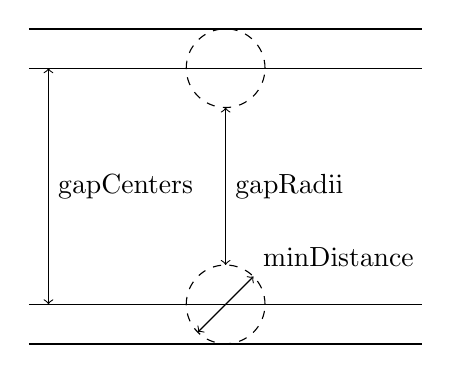
\begin{tikzpicture}
        \pgfmathsetmacro{\wallLength}{5}
        \pgfmathsetmacro{\gap}{4}
        \pgfmathsetmacro{\minDistance}{1}
        \pgfmathsetmacro{\labelOffset}{0.25}

        \draw[thick] (-\wallLength/2, -\gap/2) -- (+\wallLength/2, -\gap/2);
        \draw[dashed] (0, -\gap/2 + \minDistance/2) circle(\minDistance/2);
        \draw (-\wallLength/2, -\gap/2 + \minDistance/2) --
            (+\wallLength/2, -\gap/2 + \minDistance/2);
        \draw[thick] (-\wallLength/2, +\gap/2) -- (+\wallLength/2, +\gap/2);
        \draw[dashed] (0, +\gap/2 - \minDistance/2) circle(\minDistance/2);
        \draw (-\wallLength/2, +\gap/2 - \minDistance/2) --
            (+\wallLength/2, +\gap/2 - \minDistance/2);

        \draw[<->] (-\wallLength/2 + \labelOffset, -\gap/2 + \minDistance/2) --
            node[right]{gapCenters} (-\wallLength/2 + \labelOffset, +\gap/2 - \minDistance/2);
        \draw[<->] (0, -\gap/2 + \minDistance) -- node[right]{gapRadii}
            (0, +\gap/2 - \minDistance);
        \begin{scope}[shift={(0, -\gap/2 + \minDistance/2)}]
            \draw[<->] (225: \minDistance/2) -- (45: \minDistance/2) node[above right]{minDistance};
        \end{scope}
    \end{tikzpicture}

\end{document}
